\documentclass[11pt]{article}
\usepackage{fontspec}
\setmainfont{NotoSerif-Regular.ttf}[Path=C:/Windows/Fonts/,ItalicFont=NotoSerif-Italic.ttf,BoldFont=NotoSerif-Bold.ttf,BoldItalicFont=NotoSerif-BoldItalic.ttf]
\usepackage[a4paper,margin=22mm]{geometry}
\usepackage{amsmath,amssymb,graphicx,xcolor,hyperref,needspace}
\usepackage[normalem]{ulem}
\let\MathUnderline\underline
\renewcommand{\underline}[1]{\ifmmode\MathUnderline{#1}\else\uline{#1}\fi}
\hypersetup{unicode=true,colorlinks=true,linkcolor=blue,pdfauthor={}}
\setlength{\parindent}{0pt}
\setlength{\parskip}{.4em}
\setlength{\emergencystretch}{3em}
\raggedright
\newcommand{\SourcePage}[2]{\par\smallskip\phantomsection\label{#1:source-page}{\small\sffamily\color{blue!55!black}#1}\par\smallskip}
\newcommand{\EvidenceBlock}[4]{%
 \par\smallskip\noindent\begin{minipage}{\linewidth}
 \begin{minipage}[t]{.47\linewidth}\vspace{0pt}\centering
 \csname evidence-#1-#2\endcsname\par
 {\scriptsize\SourceCropCaption\ #1}\par
 \end{minipage}\hfill
 \begin{minipage}[t]{.49\linewidth}\vspace{0pt}\raggedright
 {\small\color{orange!65!black}\textbf{#4} #3}\par
 \end{minipage}
 \end{minipage}\par\smallskip}
\newcommand{\Unclear}[3]{\EvidenceBlock{#1}{#2}{#3}{\ReadingCaption}}
\newcommand{\Incomplete}[3]{\EvidenceBlock{#1}{#2}{#3}{\IncompleteCaption}}
\newcommand{\SourceFigure}[3]{\EvidenceBlock{#1}{#2}{#3}{\DiagramCaption}}
\expandafter\def\csname evidence-GELFAND-P000001-module-letter\endcsname{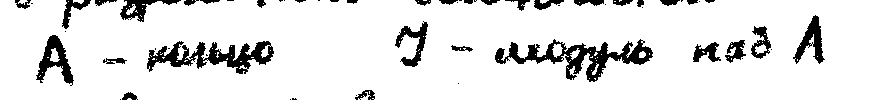
\includegraphics[width=\linewidth]{figures/gelfand-p000001-module-letter-original.png}}
\expandafter\def\csname evidence-GELFAND-P000001-diagram-blowup\endcsname{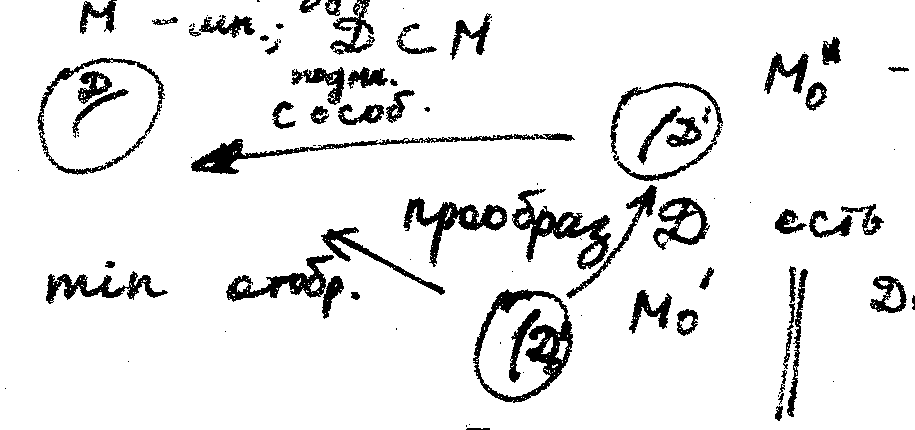
\includegraphics[width=\linewidth]{figures/gelfand-p000001-diagram-blowup-original.png}}
\expandafter\def\csname evidence-GELFAND-P000001-blowup-notation\endcsname{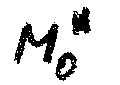
\includegraphics[width=.43\linewidth]{figures/gelfand-p000001-upper-blowup-label-original.png}\hfill
\includegraphics[width=.50\linewidth]{figures/gelfand-p000001-lower-blowup-label-original.png}}
\expandafter\def\csname evidence-GELFAND-P000001-origin-example\endcsname{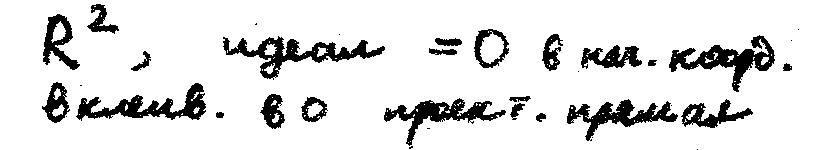
\includegraphics[width=\linewidth]{figures/gelfand-p000001-origin-example-original.png}}
\newcommand{\SourceCropCaption}{Оригинальные фрагменты:}\newcommand{\ReadingCaption}{Сомнительное чтение.}\newcommand{\IncompleteCaption}{Неразобранный фрагмент.}\newcommand{\DiagramCaption}{Рисунок и набранное описание.}
\hypersetup{pdftitle={Семинар И. М. Гельфанда — глава 1}}
\begin{document}
{\large\bfseries Семинар И. М. Гельфанда — глава 1}\par
{\small Начало читательского издания. Исходный кадр 1. Текст и формулы набраны; оригинальные фрагменты показаны при каждом сомнительном чтении. Рабочий фрагмент, не вся глава.}\par\medskip
\SourcePage{GELFAND-P000001}{unlabelled}
Понед. $21/\mathrm{IX}$.
Декартовы и булевы произв. групп.

«Хиронака: о разрешении особенностей».
\underline{Гельфанд}

$A$ — кольцо, $\mathcal{J}$ — модуль над $A$.
\Unclear{GELFAND-P000001}{module-letter}{Буква модуля и идеала передана как $\mathcal{J}$; возможны $\mathcal{I}$ или $J$.}

Раздутие — ?
$M$ — мн.; $D\subset M$.
[Под $D$:] подмн. с особ.

$M_0^H$ — раздутие. Blowing-up.
Прообраз $D$ есть $D'$ мн. разм. $n-1$.
$D_0$ — $(n-1)$-мерное.
\SourceFigure{GELFAND-P000001}{diagram-blowup}{Три обведённых рисунка: слева область с $D$, справа сверху область с $D'$ и подписью $M_0^H$, справа снизу область и подпись $M'_0$. Верхняя стрелка направлена влево; нижняя наклонная стрелка также влево, с подписью «непр. отобр.». Точные внутренние кривые, подписи и соединение нижней области с верхней требуют сравнения со сканом.}
\Unclear{GELFAND-P000001}{blowup-notation}{Верхний индекс у $M_0$ похож на $H$; подпись нижней области похожа на $M'_0$.}

Конструкция — Гротендик.
$A$ — кольцо, $\mathcal{J}$ — модуль.
\underline{Прим.} $A$ — кольцо ф-й;
$\mathcal{J}$ — идеал ф-й, обр. в $0$ на $D$.

Получится пучок колец и пучок модулей.
$A$ — кольцо, $\mathcal{J}$ — идеал.
Построим $X$, $O_X$ — пучок колец,
$\mathcal{J}_X$ — пучок идеалов, чтобы
\begin{gather*}
 (A,\mathcal{J})\ \longleftarrow\ (X,O_X,\mathcal{J}_X).
\end{gather*}
[Под стрелкой:] лин. отобр.

$(A,\mathcal{J})$ — пучок, порожд. $1$-м ид.

$\mathcal{J}_X$ обратим, т. е. идеал кольца:
$\exists f\in\mathcal{J}_X$ такого, что $O_Xf=\mathcal{J}_X$.
[Над формулой, стрелка к $\exists$:] образ.

(Идеал — главный, если $\mathcal{J}$ — идеал.)
Тогда многообр. нулей — $1$ ур-е.

$A$ — кольцо, $\mathcal{J}$ — идеал.
\underline{Тип. пример:} $R^2$, идеал $=0$ в нач. коорд.
\Unclear{GELFAND-P000001}{origin-example}{Следующая строка: «Вклеив. в $0$ проект. прямой»; начало может читаться «Оклеив.».}

$A$, $\mathcal{J}$ — мод.
\begin{gather*}
 \mathcal{J}\otimes_A\mathcal{J},\qquad
 \mathcal{J}\otimes_A\mathcal{J}\otimes_A\mathcal{J},\ldots
\end{gather*}
[Над группами тензорных произведений:] симм.; симм.

Рассм. форм. суммы
\begin{gather*}
 \sum_{k=0}^{N}a_kz^k.
\end{gather*}
Склад. и умн.
$x\otimes y=y\otimes x$.
\begin{gather*}
 a_0\in A,\qquad a_1\in\mathcal{J},\qquad
 a_2\in\mathcal{J}\otimes_A\mathcal{J}\quad\text{—}
\end{gather*}



\clearpage\section*{Полные примечания к чтениям}
\subsection*{GELFAND-0001-U001}
\EvidenceBlock{GELFAND-P000001}{module-letter}{После A — кольцо стоит рукописная буква с развилкой сверху и нижним крюком; она повторяется у модуля и идеала.}{Наблюдение.}
\textbf{Варианты: } \(\mathcal{J}\); \(\mathcal{I}\); J\par
\textbf{Историческая помета: } В тексте использован каллиграфический J как графический кандидат; обозначение не определено по математическому смыслу.\par
\textbf{Повторное сравнение: } В трёх отдельных вхождениях при 5×/10× видны развилка сверху и нижний крюк. Это подтверждает единое графическое обозначение,но не устанавливает однозначно условное различие I/J.\par
\subsection*{GELFAND-0001-U002}
\EvidenceBlock{GELFAND-P000001}{diagram-blowup}{В верхней половине три округлых контура с внутренними кривыми, две стрелки влево; над ними и рядом D, D', M и индексы.}{Наблюдение.}
\textbf{Варианты: } Не предложены.\par
\textbf{Историческая помета: } Неуверенные внутренние кривые и соединения не перерисованы. Описание и описание исходного рисунка сохраняют источник для проверки.\par
\textbf{Повторное сравнение: } Полная вырезка рисунка теперь показана при его набранном описании. Видны оба наконечника стрелок влево. От нижнего контура вверх к области около D идёт отдельный изогнутый штрих; его точное соединение с верхним контуром не утверждается.\par
\subsection*{GELFAND-0001-U003}
\EvidenceBlock{GELFAND-P000001}{blowup-notation}{Верхний индекс у \(M_0\) выглядит как H; у нижней области над \(M_0\) стоит короткий штрих.}{Наблюдение.}
\textbf{Варианты: } \(M_0^H\); \(M'_0\); \(M_0^N\); \(M'_0\)\par
\textbf{Историческая помета: } Индексы и штрих требуют сравнения с оригиналом.\par
\textbf{Повторное сравнение: } Непосредственно при чтении помещены отдельные крупные вырезки тёмного верхнего индекса и нижнего штриха. Нижний штрих различим; для тёмного верхнего знака нет достаточного основания исключить N в пользу H.\par
\subsection*{GELFAND-0001-U006}
\EvidenceBlock{GELFAND-P000001}{origin-example}{Справа от примера \(R^2\) строка начинается связной группой букв и оканчивается в 0 проект. прямой.}{Наблюдение.}
\textbf{Варианты: } Вклеив. в 0 проект. прямой; Оклеив. в 0 проект. прямой\par
\textbf{Историческая помета: } Фраза дана внутри пометы сомнительного чтения, без выбора по смыслу раздутия.\par
\textbf{Повторное сравнение: } Широкий контекст и детали 5×/10× существенно поддерживают начальную В и сокращение «Вклеив.». Исторический вариант сохранён; формулировка не заменена стандартным определением раздутия.\par
\end{document}
